%!TEX encoding = UTF-8 Unicode
%!TEX program = xelatex

\documentclass[bachelor]{ustcthesis}
% bachelor|master|doctor
\usepackage{ustcextra}
\graphicspath{{figures/}}
\bibliographystyle{ustcauthoryear}
% \bibliographystyle{ustcnumerical}

\renewpagestyle{front}[\zihao{-5}]{
    \sethead{}{即时通讯系统概要设计}{}
    \setfoot{}{\thepage}{}
    \headrule
}
\renewpagestyle{main}[\zihao{-5}]{
    \sethead{}{即时通讯系统概要设计}{}
    \setfoot{}{\thepage}{}
    \headrule
}
\newcommand{\HRule}{\rule{\linewidth}{0.5mm}}
\newcommand{\tabincell}[2]{\begin{tabular}{@{}#1@{}}#2\end{tabular}}

\begin{document}



\begin{titlepage}
\begin{center}
~\\[5cm]
\HRule \\[0.4cm]
{\huge \bfseries 即时通讯系统\\概要设计}\\[0.4cm]
\HRule \\[1.5cm]

\begin{tabular}{ccc}
      & 人员 & 日期 \\ 
      &  戴路  &  \\ 
拟制  &  张劲暾 & 2019-05-12 \\ 
      &  王浩宇 &  \\ 
评审人 & • & • \\ 
批准 & • & • \\ 
签发 & • & • \\ 
\end{tabular} 

\end{center}
\end{titlepage}



\frontmatter
\begin{abstract}
%================== 摘要 ===============================
本文档是一份即时通讯系统的设计概要,包括即时通讯系
统的任务概述、总体设计、接口设计、数据结构设计、数据库设计、界面设计、
出错处理设计和维护设计等详细描述。本文档可以为项目开发和维护人员提供参考手册。本文档的预期读者为系统设计人员、软件开发人员、客户方的系统设计人员和项目评审人员。


\textbf{关键词:} 即时通讯系统\quad 团队工作\quad 设计\quad 开发\quad Java\quad 网络通信 \quad
%=======================================================
\begin{table}[htbp]
\centering
\caption{缩略词清单} \label{tab:simpletable}
\begin{tabular}{|c|c|c|}
    \hline
    缩略语 & 英文全名 & 中文解释 \\
    \hline
    CPU & Central Processing Unit & 中央处理器\\
    \hline
    API & Application Programming Interface & 应用程序编程接口\\
    \hline
    DB & Database & 数据库 \\
    \hline
\end{tabular}
\end{table}
%=======================================================
\end{abstract}

\tableofcontents
\listoffigures
\listoftables
% \listofalgorithms  % 算法索引,如不需要,可直接注释掉本行
% \begin{notation}

%\centering
%XX 软件需求规格说明书

%关键词:能够体现文档描述内容主要方面的词汇。
 
%摘要:


\centering
\begin{tabular}{rl}
$\ln x$ & natural logarithm $\log_ex$ \\
$\log x$ & common logarithm $\log_{10}x$ \\
$x\ \mathrm{mod}\ y$ & remainder \\
\end{tabular}

\end{notation}


\mainmatter
\chapter{简介}
\section{目的}
% This section should state the purpose of the document. It could also specify the intended audience. Identify the product whose software requirements are specified in this document.

% 这部分要描述文档的目的。应该指明读者。说明本需求文档描述了哪个产品的软件需求。

现代工作团队,包括高校学生团体,课堂组织,班级管理,科研团队,企业部门,开发团队,工作小组等对于即时通讯系统
有着专业的、高质量的应用需求。能够提供高效、专业、功能强大、扩展性好的即时通讯系统对于提高
工作团队工作效率和管理水平有着重要意义。本产品将降低信息管理和通讯代价,为不同情境下的即时通讯需求
提供解决方案,包括对于一对一即时通讯(私聊)功能、情境群聊功能、个人日程管理、活动/任务发布,音视频通话/会议、
广播/公告板功能,个性化好友推荐,在线文档写作平台等工作团队需求度较高的需求的解决方案。

\section{范围}
% This section should address areas which this document includes and that are specifically excludes. 

% 本节应描述文档所包括和不包括的内容。
    本文档包括对于用户需求的分析和产品功能的介绍,描述各项功能的具体需求,约束和限制,流程,依赖关系,
    为即时通讯系统的设计、实现、测试以及验收提供重要依据,也为评价系统功能和性能
    提供标准。本文档可供用户、项目管理人员、系统分析人员、程序设计人员以及
    系统测试人员阅读和参考。

\chapter{总体概述}
%======================================================================================
% 本节描述影响产品和产品需求的一般因素。由以下4个部分构成。 
% 有一点需说明的是本节不描述具体的需求,只是使那些将要描述的具体需求更易于理解。
%======================================================================================
\section{软件概述}

	\subsection{项目介绍}
	%======================================================================================
	% 描述本软件需求所描述的项目的背景。
	% 例如:本项目是一系列版本中的一个,或者是替代某个已经存在的系统,还是一个新的独立的项目。
	%======================================================================================
	本项目是一个新的独立的项目,旨在为现代高校和企业工作团队提供一个完整高效的即时通讯系统平台;
	实现通讯,管理,公告,文件的在线支持;
	使得工作团队可以随时随地交流信息,协同合作;
	方便团队的组织和事务、活动信息的发布;
	为个人资料管理和日程安排提供高效工具。

	\subsection{产品环境介绍}
	%=========================================gongnneg=============================================
	% 描述的是本产品与其它产品或项目所组成的整体环境。
	% 1.如果本产品是独立的并完全自我包含,在此说明这一点。
	% 2.如果SRS定义的产品是更大的系统或项目的组件(此种情形经常发生),那么应:
	%	A. 	描述此大系统或项目每个组件的功能,并且标识接口。
	%	B. 	确定本软件产品主要外部接口。
	%		(注意:在此部分并不进行这些接口的详细描述;对这些接口的详细描述在SRS的其它部分提供。)
    %	C. 	描述相关产品硬件和所使用的外部设备。(注意:这只是概述性描述。)
	% 通过方块图来描述大系统或项目的主要组件,互连性以及外部接口将是非常有帮助的。
	% 本部分不应提出一个具体的设计解决方案或对解决方案的具体设计约束(具体设计约束将在具体需求章节中描述)。
	% 本部分内容是产生设计约束的基础。
	%======================================================================================
	本产品是一个相对独立的的产品,可以独立运行实现绝大多数核心功能需求,
	扩展性功能进一步支持邮箱管理,需要的其他组件是邮箱组件,包括登录认证,接收邮件和发送邮件
	功能接口,不需要其他外部设备。
\newpage
\section{软件功能}
%======================================================================================
% 概述软件的必须实现的和通过用户操作实现的主要功能。
% 这里只需要进行简要描述(例如目录列表),详细描述在详细需求部分描述。
% 对需求功能进行组织,以便于读者理解,并能指导后续的设计和测试。
% 可以用图表来表示主要需求群组之间的关系,例如:高层的数据流图,面向对象的分析等。
% 有时此部分所要求的功能概述可以从分配具体功能给此软件产品的更高层规格(如果存在的话)直接引用。
% 本节不应描述具体需求。但本节内容是具体需求章节的基础。
%======================================================================================
\begin{center}
	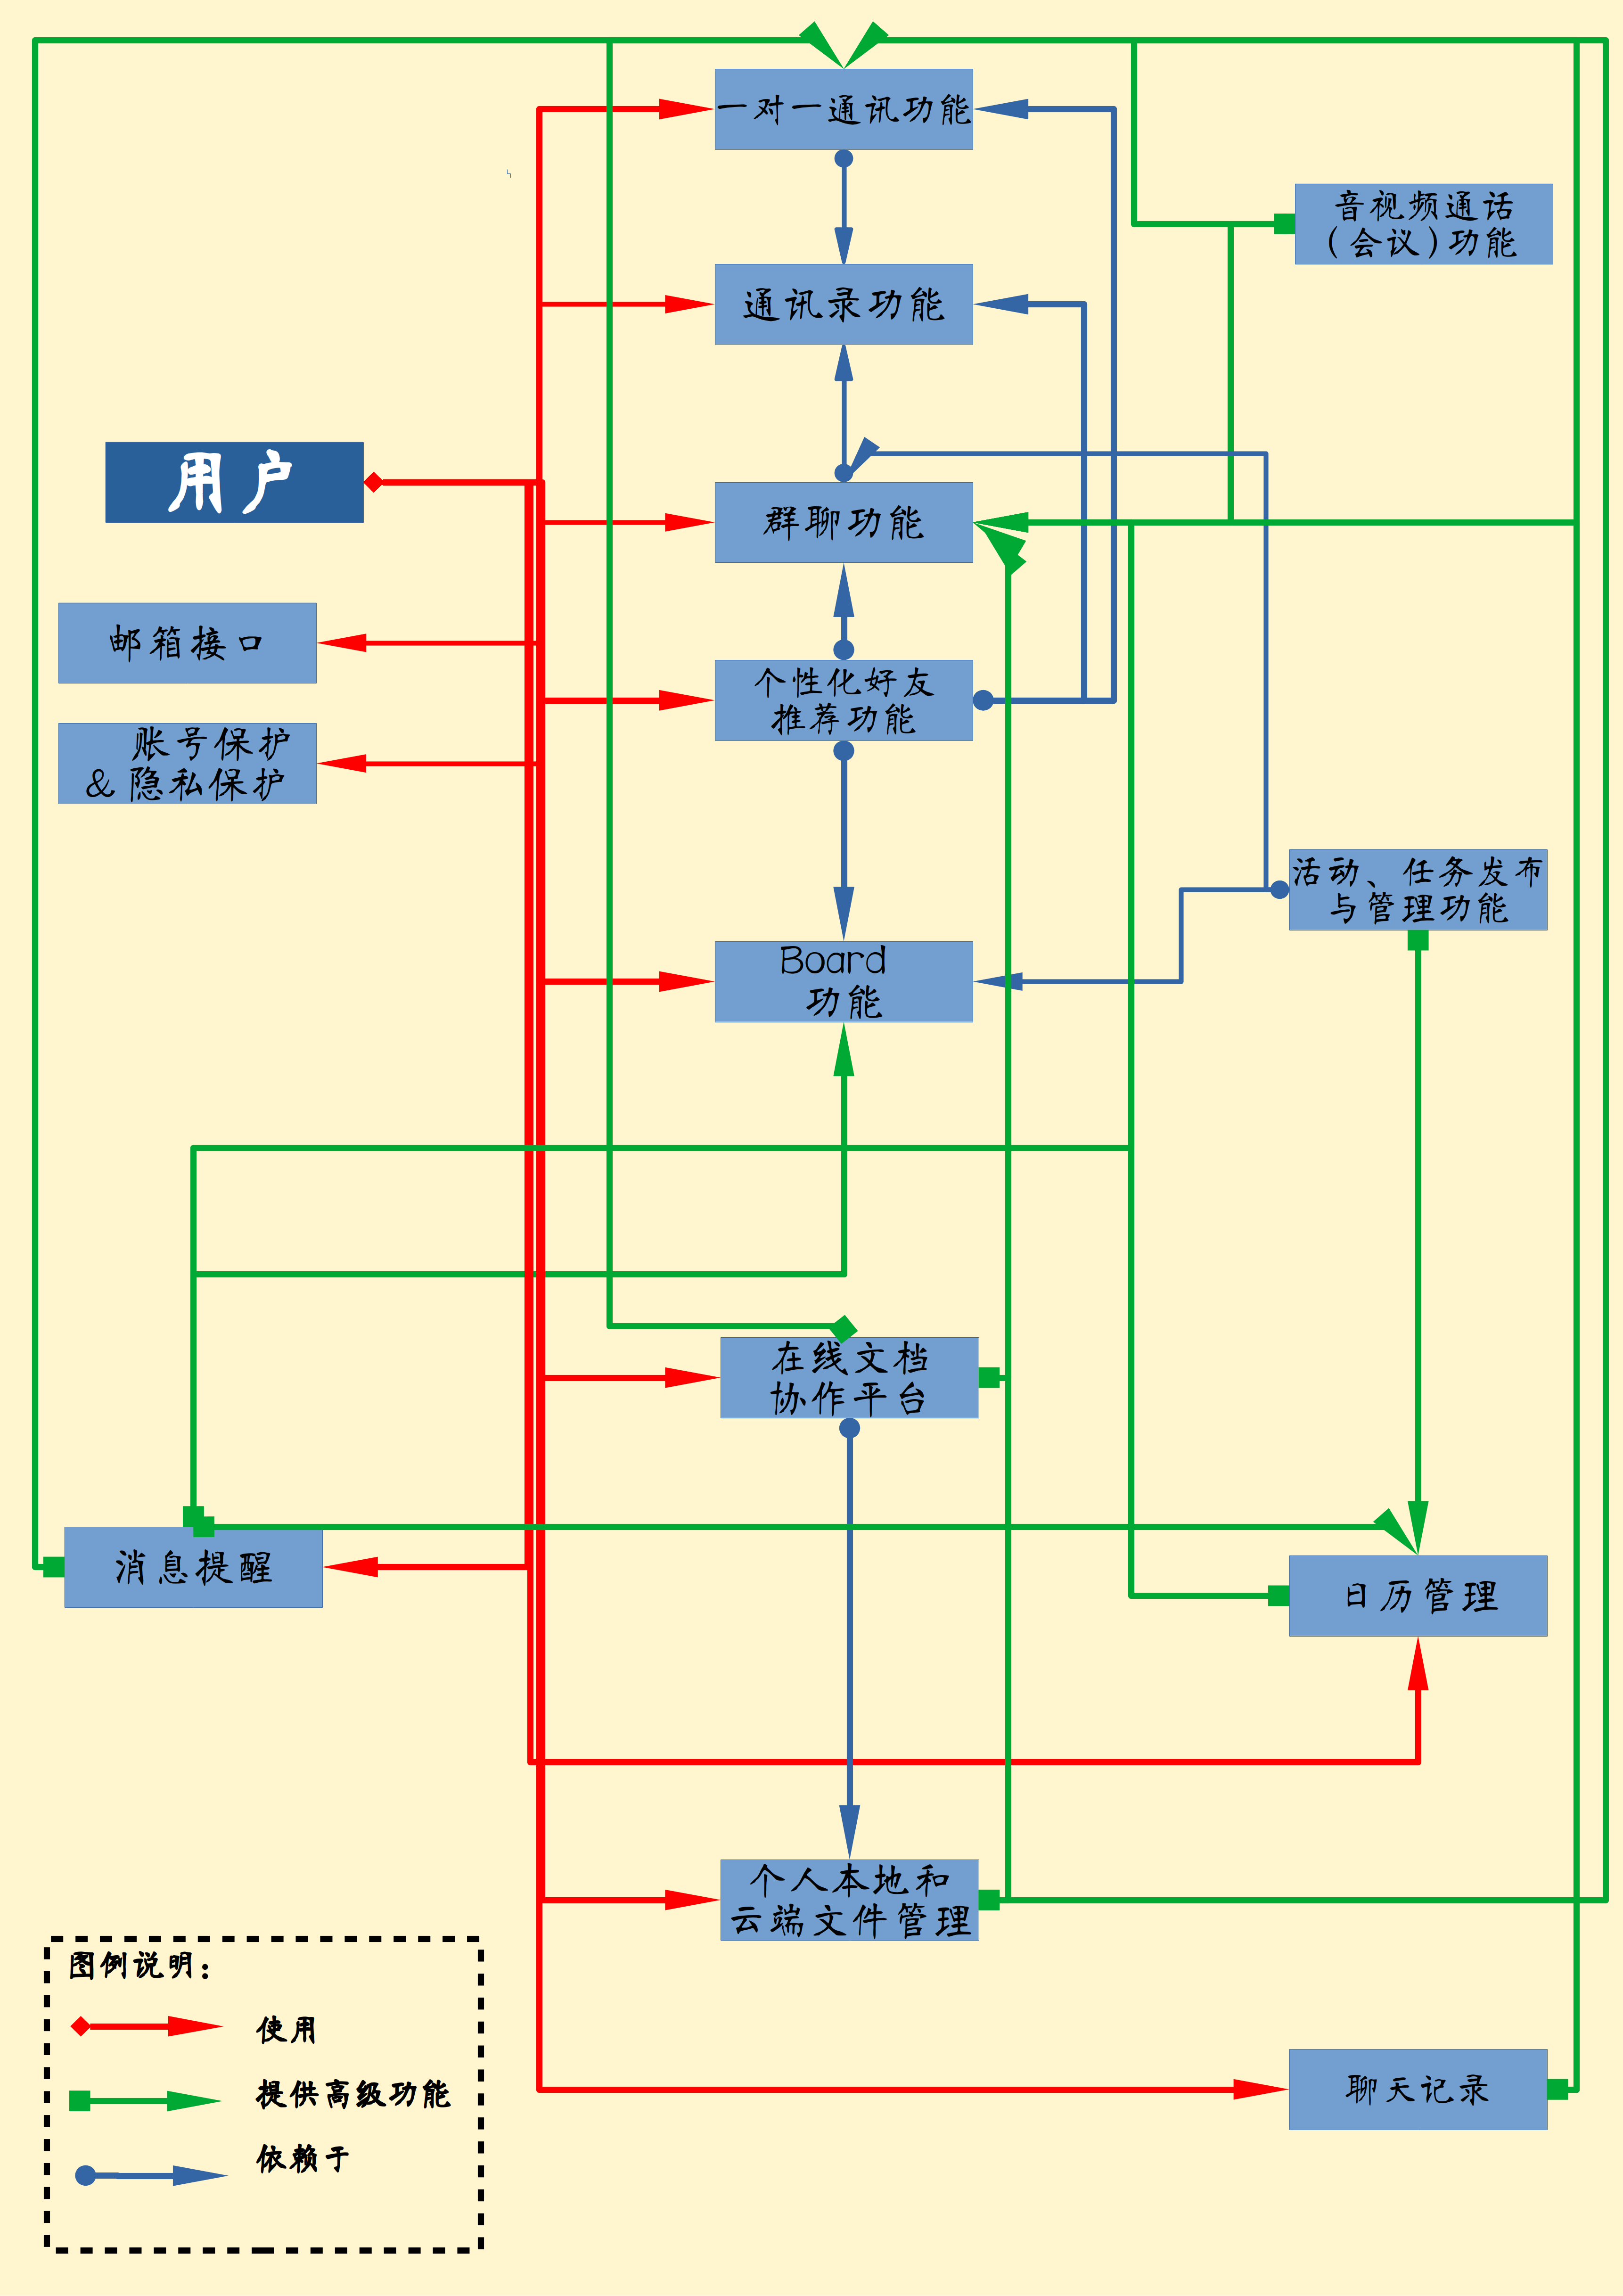
\includegraphics[scale = 0.75]{chat.png}
\end{center}
\section{用户特征}
%======================================================================================
% 列出对用户或系统操作者的要求,如:经验,能力,角色等。
% 本节不应描述具体需求。但本节内容是具体需求章节的基础。
%======================================================================================
\noindent
	本软件的主要目标人群包括:
	\begin{itemize}
		\item 高校大学生
		\item 科研机构研究人员
		\item 企业部门人员
		\item 工程开发团队人员
	\end{itemize}
	它主要适用于具有如下特点的人员:
	\begin{itemize}
		\item 在短期稳定的组织,如班级,实验室,团队
		\item 组织需要合作或者布置任务
		\item 需要合作编辑文档
		\item 需要频繁的信息沟通
		\item 定期开会
		\item 通信环境中有很多文件需要交换,发布、处理
		\item 有一些任务需要按时完成
		\item 日程安排严谨
		\item 对于所在环境(校园,公司)有社交需求
		\item 需要一定的通讯信息安全保证
		\item 有频繁、重要的邮件需要处理
	\end{itemize}
	针对以上用户特点,本软件可以高效,专业、全面地提供即时通讯及配套的各种功能。
\section{假设和依赖关系}
%======================================================================================
% 列出可能影响SRS中需求的所有的假设因素(与已知事实相对而言),
% 包括准备使用的第三方或商业组件,操作和开发环境的问题约束等。
% 如果上述假设不正确、没有被告知或者改变了都将对项目产生影响。
% 列出项目对外部条件的依赖,例如重用其他项目的模块等。
% 如果在其他文档(例如项目计划或范围文档等)里已经描述了,在这里可以不用描述。
%======================================================================================
\begin{itemize}                                                      
	\item 操作平台:Android,IOS,Windows,Linux
	\item 内部依赖关系:\\
		一对一通讯系统功能依赖于通讯录功能\\
		群聊功能依赖于通讯录功能\\
		个性化好友推荐功能依赖于一对一通讯功能、群聊功能、通讯录功能和Board功能\\
		在线文档协作平台依赖于个人文件和云端文件管理功能\\
		活动、任务发布与管理功能依赖于群聊功能和Board功能
	\item 外部依赖关系:\\
		邮箱接口功能依赖于外部邮箱组件
	\item 服务器端:借助第三方服务器
\end{itemize}
\chapter{总体设计}
\section{软件描述}
系统包括前台和后台两个部分。

前台主要功能是:

后台主要功能是:

\section{处理流程}
\subsection{总体流程}
此处应当有一个图和对应的描述。

\subsection{系统基本流程}
此处应当有一个图和对应的描述。

\subsection{客户端基本流程}
这只是举个例子,如果没有客户端则不需要此节。

\subsection{服务器端基本流程}
这只是举个例子,如果没有服务器端则不需要此节。

\subsection{功能1具体流程}
举个例子:交易处理流程

已登录用户在购物车中提交请求交易的 POST 请求,提交的表单中指明了交易中包括的
所有商品、商家、付款信息、收货地址,输入输出处理系统接收到合法请求后,向商品信息
系统请求数据,收到数据以后验证是否正确,然后向订单系统发起生成新订单的请求,订单
系统负责更新商品信息系统、商家信息,通知商家接单,返回订单处理结果输入输出处理系
统,输入输出处理系统依照结果产生 HTML 页面,并返回给用户。

\subsection{功能2具体流程}
此处应当有描述。

\subsection{功能3具体流程}
此处应当有一个描述。



\section{功能结构设计}
\subsection{整体结构}
此处应当有一个图和对应的描述。系统如果像微内核那样,划分成核心模块和若干个子系统,此处应当有图示及说明,然后后续几个节应当描述这几个子系统。如果系统像宏内核,那应当说明有哪些紧密联系的模块,并在后续几个节内描述这些模块。

\subsection{用户端结构}
此处应当有一个图和对应的描述。这只是举个例子。可能的内容包括用户端的具体模块、耦合情况等。

\subsection{服务器端结构}
此处应当有一个图和对应的描述。这只是举个例子。

\subsection{后台数据库维护模块结构}
此处应当有一个图和对应的描述。这只是举个例子。



\section{功能需求与程序代码的关系}
[此处指的是不同的需求分配到哪些模块去实现。可按不同的端拆分此表]
\begin{table}[htbp]
\centering
\caption{功能需求与程序代码的关系表} \label{tab:requirement-module}
\begin{tabular}{|c|c|c|c|}
    \hline
    · & 模块1 & 模块2 & 模块3 \\
    \hline
    需求1 & · & Y & · \\
    \hline
    需求2 & · & Y & · \\
    \hline
    需求3 & · & Y & · \\
    \hline
    需求4 & Y & · & · \\
    \hline
    需求5 & · & · & Y \\
    \hline
\end{tabular}
\note{各项功能需求的实现与各个程序模块的分配关系}
\end{table}
\chapter{接口设计}
\section{外部接口}
比如说需要用到支付宝等外部支付系统,接口应当如何封装。

\subsection{支付宝接口}
详细讲述不同的接口(查询状态、支付交易、获取回执等)

\section{内部接口}
内部模块/系统之间的交互的接口。
\chapter{数据结构设计}
\section{逻辑结构设计}
\subsection{用户管理系统数据结构设计}
讲述本系统内需要什么数据结构。这指的是程序运行过程中维护的数据结构。只是举个例子,此处应和3.3一致。
\subsection{客户端数据结构}

\subsection{用户端数据结构}

\section{物理结构设计}
各数据结构无特殊物理结构要求。(如果有,比如说hadoop等,应当具体说明)

\section{数据结构与程序模块的关系}
[此处指的是不同的数据结构分配到哪些模块去实现。可按不同的端拆分此表]
\begin{table}[htbp]
\centering
\caption{数据结构与程序代码的关系表} \label{tab:datastructure-module}
\begin{tabular}{|c|c|c|c|}
    \hline
    · & 模块1 & 模块2 & 模块3 \\
    \hline
    结构1 & · & Y & · \\
    \hline
    结构2 & · & Y & · \\
    \hline
    结构3 & · & Y & · \\
    \hline
    结构4 & Y & · & · \\
    \hline
    结构5 & · & · & Y \\
    \hline
\end{tabular}
\note{各项数据结构的实现与各个程序模块的分配关系}
\end{table}
\chapter{数据库设计}
\section{数据库环境说明}
本系统的数据系统采用MySQL/PostgreSQL/Microsoft SQL Server数据库系统。

其中xxx模块因为xxx而需要用到Hadoop架构。

\section{数据库的命名规则}
是否允许单词缩写,允许的单词缩写有哪些。

表名是单数还是复数。关联表如何命名。字符数限制等。

字段是否带上前缀(如integer类型则加上i前缀等)。

\section{逻辑设计}
是否需要满足某一种范式。

画个实体的逻辑关系表/图在此处。

\section{物理设计}
\subsection{数据库产品}
用哪家数据库,是否分布式等。
\subsection{实体属性、类型、精度}
\subsubsection{客户数据表设计}
\begin{table}[htbp]
\centering
\caption{用户数据表Users设计} \label{tab:client-database}
\begin{tabular}{|c|c|c|c|c|}
    \hline
    字段名 & 类型 & 大小 & 说明 & 备注 \\
    \hline
    ID & char & 64 & 用户的唯一标识符 & 主键\\
    \hline
    pw & char & 512 & 用户的登录密码 & · \\
    \hline
\end{tabular}
\note{用户数据表Users设计}
\end{table}

\subsubsection{订单数据表设计}
\begin{table}[htbp]
\centering
\caption{订单数据表Orders设计} \label{tab:order-database}
\begin{tabular}{|c|c|c|c|c|}
    \hline
    字段名 & 类型 & 大小 & 说明 & 备注 \\
    \hline
    ID & char & 64 & 订单的唯一标识符 & 主键\\
    \hline
    user & char & 64 & 对应用户 & 外键,来自xx表 \\
    \hline
\end{tabular}
\note{订单数据表Orders设计}
\end{table}
\section{安全性设计}
备份和容灾设计。

\section{数据库管理与维护说明}
对于数据库的维护,随时对数据库中的信息加以调试和保存备份。同样需要个工作人员进行系统的分析和用户的反馈,对系统进行升级以及功能的完善。同时保证系统安全有序的运行。
\chapter{界面设计}
\section{客户端界面}
此处应当有一个简略的图,重点是展示你与用户交互的逻辑。(processon上画一个不花时间)

\section{服务器端界面}
此处应当有一个简略的图。

\section{登录界面}
此处应当有一个简略的图。

\section{xxx功能界面}
此处应当有一个简略的图。

\chapter{出错处理设计}
\section{数据库出错处理}
多重备份时,应采取何种策略,先利用哪一份备份;系统是否暂停服务等。

\section{某模块失效处理}
是否整个系统暂停服务,还是维持最小服务状态、如何尽快恢复服务还是删库跑路等。
\chapter{安全保密设计}
可能的内容包括保密性、是否采取加密传输、密钥如何分发和管理等。
\chapter{维护设计}
可能的内容包括数据库的日常备份、压缩、维护等。

% \chapter{图片}
本章展示图片相关用法。

\section{示例}
\begin{figure}[ht]
\centering

\includegraphics[width=10cm]{ustc_logo_fig}
\caption{测试图片} \label{fig:figure1}
\end{figure}

\section{带图注的图}
\begin{figure}[ht]
\centering

\includegraphics[width=10cm]{ustc_logo_fig}
\caption{带图注的图片}\label{fig:noted-figure}
\note{the solid lines represent the time histogram of the spontaneous activities of an old monkey cell(gray) and a young monkey cell (black). The bin-width is 1}
\end{figure}

% \chapter{表格}

\section{A Simple Table}
\begin{table}[htbp]
\centering
\caption{这里是表的标题} \label{tab:simpletable}
\begin{tabular}{|c|c|}
    \hline
    a & b \\
    \hline
    c & d \\
    \hline
\end{tabular}
\note{这里是表的注释}
\end{table}

\section{长表格}
\begin{longtable}{ccc}
% 首页表头
\caption[长表格演示]{长表格演示} \label{tab:longtable} \\
\toprule[1.5pt]
名称  & 说明 & 备注\\
\midrule[1pt]
\endfirsthead
% 续页表头
\caption[]{长表格演示(续)} \\
\toprule[1.5pt]
名称  & 说明 & 备注 \\
\midrule[1pt]
\endhead
% 首页表尾
\hline
\multicolumn{3}{r}{\small 续下页}
\endfoot
% 续页表尾
\bottomrule[1.5pt]
\endlastfoot

AAAAAAAAAAAA   &   BBBBBBBBBBB   &   CCCCCCCCCCCCCC   \\
AAAAAAAAAAAA   &   BBBBBBBBBBB   &   CCCCCCCCCCCCCC   \\
AAAAAAAAAAAA   &   BBBBBBBBBBB   &   CCCCCCCCCCCCCC   \\
AAAAAAAAAAAA   &   BBBBBBBBBBB   &   CCCCCCCCCCCCCC   \\
AAAAAAAAAAAA   &   BBBBBBBBBBB   &   CCCCCCCCCCCCCC   \\
AAAAAAAAAAAA   &   BBBBBBBBBBB   &   CCCCCCCCCCCCCC   \\
AAAAAAAAAAAA   &   BBBBBBBBBBB   &   CCCCCCCCCCCCCC   \\
AAAAAAAAAAAA   &   BBBBBBBBBBB   &   CCCCCCCCCCCCCC   \\
AAAAAAAAAAAA   &   BBBBBBBBBBB   &   CCCCCCCCCCCCCC   \\
AAAAAAAAAAAA   &   BBBBBBBBBBB   &   CCCCCCCCCCCCCC   \\
AAAAAAAAAAAA   &   BBBBBBBBBBB   &   CCCCCCCCCCCCCC   \\
AAAAAAAAAAAA   &   BBBBBBBBBBB   &   CCCCCCCCCCCCCC   \\
AAAAAAAAAAAA   &   BBBBBBBBBBB   &   CCCCCCCCCCCCCC   \\
AAAAAAAAAAAA   &   BBBBBBBBBBB   &   CCCCCCCCCCCCCC   \\
AAAAAAAAAAAA   &   BBBBBBBBBBB   &   CCCCCCCCCCCCCC   \\
AAAAAAAAAAAA   &   BBBBBBBBBBB   &   CCCCCCCCCCCCCC   \\
AAAAAAAAAAAA   &   BBBBBBBBBBB   &   CCCCCCCCCCCCCC   \\
AAAAAAAAAAAA   &   BBBBBBBBBBB   &   CCCCCCCCCCCCCC   \\
AAAAAAAAAAAA   &   BBBBBBBBBBB   &   CCCCCCCCCCCCCC   \\
AAAAAAAAAAAA   &   BBBBBBBBBBB   &   CCCCCCCCCCCCCC   \\
AAAAAAAAAAAA   &   BBBBBBBBBBB   &   CCCCCCCCCCCCCC   \\
AAAAAAAAAAAA   &   BBBBBBBBBBB   &   CCCCCCCCCCCCCC   \\
AAAAAAAAAAAA   &   BBBBBBBBBBB   &   CCCCCCCCCCCCCC   \\
AAAAAAAAAAAA   &   BBBBBBBBBBB   &   CCCCCCCCCCCCCC   \\
AAAAAAAAAAAA   &   BBBBBBBBBBB   &   CCCCCCCCCCCCCC   \\
AAAAAAAAAAAA   &   BBBBBBBBBBB   &   CCCCCCCCCCCCCC   \\
AAAAAAAAAAAA   &   BBBBBBBBBBB   &   CCCCCCCCCCCCCC   \\
AAAAAAAAAAAA   &   BBBBBBBBBBB   &   CCCCCCCCCCCCCC   \\
AAAAAAAAAAAA   &   BBBBBBBBBBB   &   CCCCCCCCCCCCCC   \\
AAAAAAAAAAAA   &   BBBBBBBBBBB   &   CCCCCCCCCCCCCC   \\
AAAAAAAAAAAA   &   BBBBBBBBBBB   &   CCCCCCCCCCCCCC   \\
AAAAAAAAAAAA   &   BBBBBBBBBBB   &   CCCCCCCCCCCCCC   \\
AAAAAAAAAAAA   &   BBBBBBBBBBB   &   CCCCCCCCCCCCCC   \\
AAAAAAAAAAAA   &   BBBBBBBBBBB   &   CCCCCCCCCCCCCC   \\
AAAAAAAAAAAA   &   BBBBBBBBBBB   &   CCCCCCCCCCCCCC   \\
AAAAAAAAAAAA   &   BBBBBBBBBBB   &   CCCCCCCCCCCCCC   \\
\end{longtable}

% \chapter{算法环境}
模板中使用 \texttt{algorithm2e} 宏包实现算法环境。关于该宏包的具体用法,
请阅读宏包的官方文档。

\begin{algorithm}[htbp]
\SetAlgoLined
\KwData{this text}
\KwResult{how to write algorithm with \LaTeX2e }

initialization\;
\While{not at end of this document}{
    read current\;
    \eIf{understand}{
        go to next section\;
        current section becomes this one\;
    }{
        go back to the beginning of current section\;
    }
}
\caption{算法示例1}
\label{algo:algorithm1}
\end{algorithm}

\IncMargin{1em}
\begin{algorithm}
\SetKwData{Left}{left}\SetKwData{This}{this}\SetKwData{Up}{up}
\SetKwFunction{Union}{Union}\SetKwFunction{FindCompress}{FindCompress}
\SetKwInOut{Input}{input}\SetKwInOut{Output}{output}

\Input{A bitmap $Im$ of size $w\times l$}
\Output{A partition of the bitmap}
\BlankLine
\emph{special treatment of the first line}\;
\For{$i\leftarrow 2$ \KwTo $l$}{
    \emph{special treatment of the first element of line $i$}\;
    \For{$j\leftarrow 2$ \KwTo $w$}{\label{forins}
        \Left$\leftarrow$ \FindCompress{$Im[i,j-1]$}\;
        \Up$\leftarrow$ \FindCompress{$Im[i-1,]$}\;
        \This$\leftarrow$ \FindCompress{$Im[i,j]$}\;
        \If(\tcp*[h]{O(\Left,\This)==1}){\Left compatible with \This}{\label{lt}
            \lIf{\Left $<$ \This}{\Union{\Left,\This}}
            \lElse{\Union{\This,\Left}}
        }
        \If(\tcp*[f]{O(\Up,\This)==1}){\Up compatible with \This}{\label{ut}
        \lIf{\Up $<$ \This}{\Union{\Up,\This}}
        \tcp{\This is put under \Up to keep tree as flat as possible}\label{cmt}
        \lElse{\Union{\This,\Up}}\tcp*[h]{\This linked to \Up}\label{lelse}
        }
    }
    \lForEach{element $e$ of the line $i$}{\FindCompress{p}}
}
\caption{算法示例2}\label{algo_disjdecomp}
\label{alog:algorithm2}
\end{algorithm}\DecMargin{1em}

% \chapter{代码环境}
模板中使用 \texttt{listings} 宏包实现代码环境。详细用法见宏包的官方说明文档。

以下是代码示例,可以在文中任意位置引用\autoref{first-code} 。
\begin{lstlisting}[language=C, caption=示例代码, label={code:first-code}]
#include <stdio.h>

int main( )
{
    printf("hello, world\n");
    return 0;
}
\end{lstlisting}

% \chapter{引用文献标注}

\section{著者-出版年制标注法}

\noindent
\verb|\citestyle{ustcauthoryear}|
\citestyle{ustcauthoryear}

\noindent
\begin{tabular}{l@{\quad$\Rightarrow$\quad}l}
  \verb|\cite{knuth86a}| & \cite{knuth86a}\\
  \verb|\citet{knuth86a}| & \citet{knuth86a}\\
  \verb|\citet[chap.~2]{knuth86a}| & \citet[chap.~2]{knuth86a}\\[0.5ex]
  \verb|\citep{knuth86a}| & \citep{knuth86a}\\
  \verb|\citep[chap.~2]{knuth86a}| & \citep[chap.~2]{knuth86a}\\
  \verb|\citep[see][]{knuth86a}| & \citep[see][]{knuth86a}\\
  \verb|\citep[see][chap.~2]{knuth86a}| & \citep[see][chap.~2]{knuth86a}\\[0.5ex]
  \verb|\citet*{knuth86a}| & \citet*{knuth86a}\\
  \verb|\citep*{knuth86a}| & \citep*{knuth86a}\\
\end{tabular}

\noindent
\begin{tabular}{l@{\quad$\Rightarrow$\quad}l}
  \verb|\citet{knuth86a,tlc2}| & \citet{knuth86a,tlc2}\\
  \verb|\citep{knuth86a,tlc2}| & \citep{knuth86a,tlc2}\\
  \verb|\cite{knuth86a,knuth84}| & \cite{knuth86a,knuth84}\\
  \verb|\citet{knuth86a,knuth84}| & \citet{knuth86a,knuth84}\\
  \verb|\citep{knuth86a,knuth84}| & \citep{knuth86a,knuth84}\\
\end{tabular}

\section{顺序编码制标注法}

\noindent
\verb|\citestyle{ustcnumerical}|
\citestyle{ustcnumerical}

\noindent
\begin{tabular}{l@{\quad$\Rightarrow$\quad}l}
  \verb|\cite{knuth86a}| & \cite{knuth86a}\\
  \verb|\citet{knuth86a}| & \citet{knuth86a}\\
  \verb|\citet[chap.~2]{knuth86a}| & \citet[chap.~2]{knuth86a}\\[0.5ex]
  \verb|\citep{knuth86a}| & \citep{knuth86a}\\
  \verb|\citep[chap.~2]{knuth86a}| & \citep[chap.~2]{knuth86a}\\
  \verb|\citep[see][]{knuth86a}| & \citep[see][]{knuth86a}\\
  \verb|\citep[see][chap.~2]{knuth86a}| & \citep[see][chap.~2]{knuth86a}\\[0.5ex]
  \verb|\citet*{knuth86a}| & \citet*{knuth86a}\\
  \verb|\citep*{knuth86a}| & \citep*{knuth86a}\\
\end{tabular}

\noindent
\begin{tabular}{l@{\quad$\Rightarrow$\quad}l}
  \verb|\citet{knuth86a,tlc2}| & \citet{knuth86a,tlc2}\\
  \verb|\citep{knuth86a,tlc2}| & \citep{knuth86a,tlc2}\\
  \verb|\cite{knuth86a,knuth84}| & \cite{knuth86a,knuth84}\\
  \verb|\citet{knuth86a,knuth84}| & \citet{knuth86a,knuth84}\\
  \verb|\citep{knuth86a,knuth84}| & \citep{knuth86a,knuth84}\\
  \verb|\cite{knuth86a,knuth84,tlc2}| & \cite{knuth86a,knuth84,tlc2}\\
\end{tabular}

\section{其他形式的标注}

\noindent
\begin{tabular}{l@{\quad$\Rightarrow$\quad}l}
  \verb|\citealt{tlc2}| & \citealt{tlc2}\\
  \verb|\citealt*{tlc2}| & \citealt*{tlc2}\\
  \verb|\citealp{tlc2}| & \citealp{tlc2}\\
  \verb|\citealp*{tlc2}| & \citealp*{tlc2}\\
  \verb|\citealp{tlc2,knuth86a}| & \citealp{tlc2,knuth86a}\\
  \verb|\citealp[pg.~32]{tlc2}| & \citealp[pg.~32]{tlc2}\\
  \verb|\citenum{tlc2}| & \citenum{tlc2}\\
  \verb|\citetext{priv.\ comm.}| & \citetext{priv.\ comm.}\\
\end{tabular}

\noindent
\begin{tabular}{l@{\quad$\Rightarrow$\quad}l}
  \verb|\citeauthor{tlc2}| & \citeauthor{tlc2}\\
  \verb|\citeauthor*{tlc2}| & \citeauthor*{tlc2}\\
  \verb|\citeyear{tlc2}| & \citeyear{tlc2}\\
  \verb|\citeyearpar{tlc2}| & \citeyearpar{tlc2}\\
\end{tabular}

\bibliography{bib/tex}

\end{document}
